\documentclass[12pt,french]{book}
\input preambule_2013
\input philippe2013_activites
\pagestyle{empty}

\begin{document}

\TitreActivite{v.2}{Tableau de variations}

Le graphique ci-dessous indique l'altitude atteinte en fonction de la distance parcourue lors d'une promenade de $5$~km.

\begin{center}
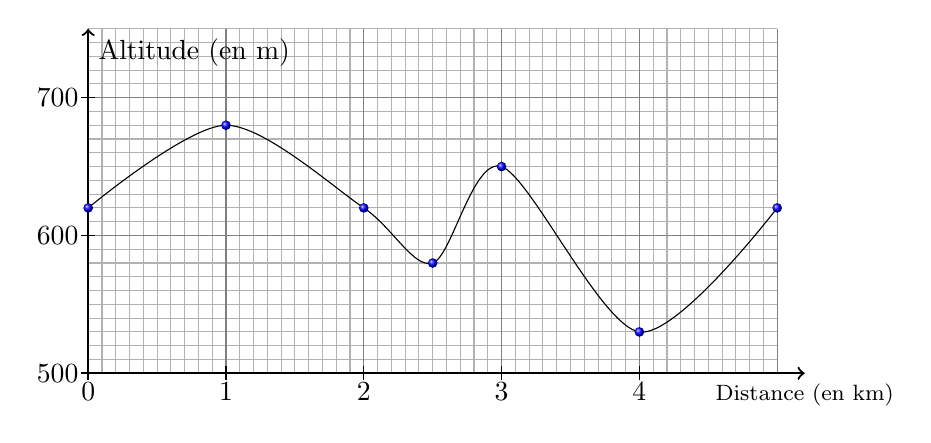
\begin{tikzpicture}[scale=1.75]
    \draw[thin,style=gray!60,step=0.1] (0,0)grid(5,2.5);
    \draw[gray] (0,0)grid(5,2.5);
    \draw[thick,->] (-0.05,0)--(5.2,0)node[below] {\footnotesize Distance (en km)};
    \draw[thick,->] (0,-0.05)--(0,2.5)node[below right] {Altitude (en m)};
    \draw plot[smooth=200,mark=ball,mark options={scale =0.5}] coordinates{(0,1.2)(1,1.8)(2,1.2)(2.5,0.8)(3,1.5)(4,0.3)(5,1.2)};
    \draw (0,0) node[left] {$500$} node[below] {$0$};
    \draw (0,1) node[left] {$600$}; \draw (0,2) node[left] {$700$};
    \draw (-0.05,1)--(0.05,1); \draw (-0.05,2)--(0.05,2);
    \draw (1,0) node[below] {$1$}; \draw (2,0) node[below] {$2$};
    \draw (3,0) node[below] {$3$}; \draw (4,0) node[below] {$4$};
    \draw (1,-0.05)--(1,0.05); \draw (2,-0.05)--(2,0.05);\draw (3,-0.05)--(3,0.05); \draw (4,-0.05)--(4,0.05);
\end{tikzpicture}
\end{center}

\begin{enumerate}
    \item Sur quels tronçons du parcours le promeneur monte-t-il ? descend-il ?
    \item Quelle est l'altitude maximale de la promenade ? l'altitude minimale ? À quelles distances ces altitudes sont-elles atteintes ?
    \item On a commencé à représenter dans un tableau les variations de l'altitude en fonction de la distance parcourue.\par Recopier et compléter le tableau ci-dessous.
        \begin{center}
            \begin{tikzpicture}
                    \tkzTabInit[espcl=2]{Distance/0.75,Altitude/2.5}{$0$,$1$,\ldots,\ldots,\ldots,$5$}
                    \tkzTabVar{-/$620$,+/$680$,,,,}
            \end{tikzpicture}
        \end{center}
    \item Quelle est l'altitude minimale pendant les trois premiers kilomètres ?
    \item Combien de fois le promeneur passe-t-il en dessous de $600$ mètres d'altitude ?
    \item La promenade peut-être être un aller-retour ? une boucle ? Justifier.
\end{enumerate}
\end{document}
